\documentclass[conference]{IEEEtran}
\IEEEoverridecommandlockouts
% The preceding line is only needed to identify funding in the first footnote. If that is unneeded, please comment it out.
%Template version as of 6/27/2024

\usepackage{cite}
\usepackage{amsmath,amssymb,amsfonts}
\usepackage{algpseudocode}
\usepackage{graphicx}
\usepackage{textcomp}
\usepackage{xcolor}
\usepackage{listings}
\usepackage{fancyvrb}
\usepackage{framed}
\usepackage{algorithm}
\usepackage{algpseudocode}
\usepackage[listings,skins]{tcolorbox}

\def\BibTeX{{\rm B\kern-.05em{\sc i\kern-.025em b}\kern-.08em
    T\kern-.1667em\lower.7ex\hbox{E}\kern-.125emX}}
\begin{document}

\title{Conference Paper Title*\\
{\footnotesize \textsuperscript{*}Note: Sub-titles are not captured for https://ieeexplore.ieee.org  and
should not be used}
\thanks{Identify applicable funding agency here. If none, delete this.}
}

\author{\IEEEauthorblockN{1\textsuperscript{st} Given Name Surname}
\IEEEauthorblockA{\textit{dept. name of organization (of Aff.)} \\
\textit{name of organization (of Aff.)}\\
City, Country \\
email address or ORCID}
\and
\IEEEauthorblockN{2\textsuperscript{nd} Given Name Surname}
\IEEEauthorblockA{\textit{dept. name of organization (of Aff.)} \\
\textit{name of organization (of Aff.)}\\
City, Country \\
email address or ORCID}
\and
\IEEEauthorblockN{3\textsuperscript{rd} Given Name Surname}
\IEEEauthorblockA{\textit{dept. name of organization (of Aff.)} \\
\textit{name of organization (of Aff.)}\\
City, Country \\
email address or ORCID}
\and
\IEEEauthorblockN{4\textsuperscript{th} Given Name Surname}
\IEEEauthorblockA{\textit{dept. name of organization (of Aff.)} \\
\textit{name of organization (of Aff.)}\\
City, Country \\
email address or ORCID}
\and
\IEEEauthorblockN{5\textsuperscript{th} Given Name Surname}
\IEEEauthorblockA{\textit{dept. name of organization (of Aff.)} \\
\textit{name of organization (of Aff.)}\\
City, Country \\
email address or ORCID}
\and
\IEEEauthorblockN{6\textsuperscript{th} Given Name Surname}
\IEEEauthorblockA{\textit{dept. name of organization (of Aff.)} \\
\textit{name of organization (of Aff.)}\\
City, Country \\
email address or ORCID}
}

\maketitle

\begin{abstract}
This document is a model and instructions for \LaTeX.
This and the IEEEtran.cls file define the components of your paper [title, text, heads, etc.]. *CRITICAL: Do Not Use Symbols, Special Characters, Footnotes, 
or Math in Paper Title or Abstract.
\end{abstract}

\begin{IEEEkeywords}
component, formatting, style, styling, insert.
\end{IEEEkeywords}

\section{Introduction}
The manual parallel implementation of numerical algorithms for modern supercomputers is often complicated. 
This is due to the increasing complexity and heterogeneity of the supercomputers which compels a numerical parallel 
program developer to deal with system parallel programming problems such as efficient load distribution, scheduling, etc. 
Otherwise, costly computational resources are wasted.
However, this is often beyond the developer's scope. This raises the problem of the automation of the numerical 
parallel programming. In order to address this problem a variety of automated parallel programming systems, languages 
and tools have been actively developed for the recent decades. 
Of interest are the tools that allow the automated construction of a parallel program for a distributed memory 
parallel computer from a numerical algorithm description. 
The following classes of such automated tools can be considered. General purpose tools are able to automatically 
construct a parallel program from any given numerical algorithm description. The price for such versatility is 
often relatively poor performance of the automatically constructed programs. On the contrary, specialized tools can 
only handle a limited class of numerical algorithms (for example, \cite{dplasma} is designed for dense linear algebra domain). 
Despite that, such specialized automated parallel program generating tools are able to employ 
domain-specific optimizations and parallel programming techniques. This often improves the constructed parallel 
programs performance significantly. However, it is clear that the problem of the automation of the numerical 
parallel programming is still far from solved.

In this paper ParSolGen (Parallel Solvers Generator), an automated parallel programs construction 
tool, is presented. ParSolGen constructs a highly efficient parallel program from a given numerical 
algorithm description written in ParSolGen language. Unlike other general purpose and domain-specific 
tools, systems and languages, ParSolGen accumulates various domain-specific 
parallel program construction algorithms and techniques within a single tool. Instead of performing 
sophisticated information dependencies analysis of the input numerical algorithm description or 
employing a general purpose run-time system approach, ParSolGen classifies the input numerical 
algorithm description. Depending on the classification result ParSolGen selects a proper domain-specific module 
that is suitable for the parallel program construction for the determined numerical algorithms class. 
This allows leveraging the advantages of domain-specific tools with the versatility approaching 
that of general purpose tools. Also such domain-specific parallel program construction modules 
accumulation enables ParSolGen to employ well-known manual parallel programming techniques 
in the automated parallel program construction.

The rest of the paper is organized as follows. Section 2 provides related work overview.

\section{Related work}
The variety of automated parallel programming tools, languages and systems have been actively developed 
for decades. General purpose run-time systems allow the automated execution of an executive representation 
of a numerical algorithm in a distributed manner. A numerical algorithm is represented as a DAG 
(Directed Acyclic Graph) of tasks with each task being associated with a user-provided implementation (kernel). 
The DAG is fed into the input of the run-time system which 
executes it on a supercomputer. Legion \cite{legion}, Charm++ \cite{charm, charm1}, QUARK \cite{quark} and 
StarPU \cite{starpu} can serve as illustrative examples of this approach. Legion uses regions (named sets of objects) concept to express data locality 
and uses those regions to describe the organization of data and information dependencies between tasks. 
Charm++ describes a numerical algorithm as a DAG of so called chares (computational tasks). Chares can communicate 
to each other by sending and receiving asynchronous messages. QUARK and 
StarPU are both task-based runtime systems allowing the one to submit tasks through the API of run-time system. 
Both systems build tasks DAG automatically and then execute it. Such general-purpose run-time systems are 
able to handle any given DAG representation of a numerical algorithm. Despite that, the tasks DAG representation 
often is not sufficient for the further classification of a numerical algorithm. This limits the 
possibilities of the accumulation of domain-specific parallel program construction modules in such systems.

There are also domain-specific languages and tools that partially automate the development of parallel 
implementations for specific classes of numerical algorithms. Halide \cite{halide} provides a domain-specific language 
allowing expressing schedules of stages of an image processing pipeline. Helide compiler is able to 
automatically construct a parallel implementation of a given image processing pipeline description. 
DPLASMA \cite{dplasma} allows the automated execution of a DAG representation of a dense linear algebra algorithm. It 
employs domain-specific DAG execution techniques which are implemented in the underlying DAGuE \cite{dague} engine. 
Such tools are not universal and can handle only a limited numerical algorithms class. Despite that, 
such systems employ domain-specific parallel program construction techniques and optimizations which 
improve the constructed parallel programs performance.

Of interest are automated parallel programming systems that combine a general purpose compiler of 
a high-level DSL and a general run-time system. Regent \cite{regent. regent1} and LuNA \cite{luna} are the examples of such systems. 
Regent compiler optimizes the input numerical algorithm description written in Regent DSL and generates 
an executable representation of it. This executive representation of the input numerical algorithm can then 
be executed by Legion run-time system. Similarly, LuNA consists of a DSL compiler and a general purpose run-time system. LuNA compiler analyzes the input algorithm description written in LuNA language and generates an executive 
representation of the input numerical algorithm which is then executed by LuNA run-time system. The systems also provide powerful means to provide specialized support of parallel program construction and execution, because execution control algorithms are excluded from the algorithm description. Thus program construction and execution can be varied freely to support efficient execution of applied algorithms in particular subject domains. The systems are therefore suitable for accumulating various system algorithms for different subject domains. 

This work extends LuNA project by providing powerful means to provide specialized support of the automated parallel program construction \cite{luna1}.  Unlike LuNA, ParSolGen language supports additional domain-specific operators (for example, vector operators such as dot-product) and types of variables, arrays and array elements. These language extensions provide the ParSolGen compiler with more information 
about the structure of the input numerical algorithm, enabling its proper classification.

\subsection{Numerical algorithm representation}
In ParSolGen algorithm is represented as a tuple of three sets (potentially infinite): a set of operations, a set of  
variables and a set of arrays. 
Variables store arbitrary data (for example: matrix blocks, vector blocks, single values, etc.). Each variable is assigned its type and an integer (version of the variable). Two different versions of a variable 
are considered as two independent variables by ParSolGen compiler. However, the values of these two variables can 
be stored within the same memory location. Variables can be aggregated into n-dimensional arrays in a manner similar to most procedural programming languages. Each operation is associated with two sets: a set of input variables and 
a set of output variables. An operation computes the values of the input variable values from the given 
values of the output variables. This is done by executing an associated sequential subroutine (kernel) 
provided by the developer of the numerical algorithm 
(for example: vector blocks multiplication, two values sum, etc.). An operation 
can be executed when all its input variable values are computed (in particular if the set of the input variables is empty). After an operation is executed 
the values of its output variables are considered computed and thus there appear other operations which can 
be executed. The algorithm description is considered executed when all operations are executed. 
In the rest of the paper, the described numerical algorithm representation is referred to as \textit{graph representation}.

An example of graph representation of the algorithm for summing vector elements is illustrated ``Fig.~\ref{fig_1}''. For 
illustrative purposes, it is illustrated as a DAG (Directed Acyclic Graph) of operations and variables. 
The edges of the DAG represent the information dependencies.
Array \textit{A} is 1-dimensional array of vector blocks each being a regular C-style 
1-dimensional array of floating point values.
Notation \textit{A\{v\}[i]} denotes an element of 1-dimensional array \textit{A} with 
index \textit{i} and version \textit{v}.

\subsection{ParSolGen language}
ParSolGen language provides convenient means of describing graph representation of numerical algorithms.
The following main statements are supported: variable, array, subroutine and 
operation declaration statements, for and while loop statements and conditional statements.
Consider the following example of the algorithm for summing two vectors described in ParSolGen.

\begin{lstlisting}[frame=single]
import init_vec(in int i, in int blockn,
	out Array<double> vec[blockn]);
import print_vec(in int i, in int blockn,
	in Array<double> x[blockn]);
import vec_sum(in int blockn,
	in Array<double> x[blockn],
	in Array<double> x1[blockn],
	out Array<double> y[blockn]);

...

int blockn = 10;
int nb = 5;

Array<double[blockn]> a[nb];
Array<double[blockn]> b[nb];
Array<double[blockn]> c[nb];

for (int i = 0; i < nb; ++i)
{
	init_vec(i, blockn, a[i]);
	init_vec(i, blockn, b[i]);
}

for (int i = 0; i < nb; ++i)
{
	vec_sum(blockn, a[i], b[i], c[i]);
}
\end{lstlisting}

Two integer variables (\textit{i} and \textit{j}) are declared. Three declared one-dimensional arrays \textit{a}, \textit{b} and \textit{c} 
consist of \textit{nb} elements. Each element is also an one-dimensional array storing \textit{blockn} double 
precision floating point values. These three arrays can be considered as blocked vectors with each one-dimensional 
block being an element of a one-dimensional ParSolGen array. 
For-loop statement is used to describe a set of operations 
each associated with kernel \textit{init\_vec} (this is done by using \textit{import} statement). 
Each operation takes values of 
\textit{i} and \textit{blockn} as input and computes the value of \textit{i}-th element of array \textit{a} (or 
\textit{b} correspondingly). These kernel call statements from so called for-loop \textit{body} (similarly, 
a body of a while loop can be considered). 
Similarly, the second for-statement describes a set of \textit{nb} operations, each 
associated with \textit{vec\_sum} kernel. These operations compute the values of the corresponding \textit{i}-th 
elements of array \textit{c} by given values of variable \textit{blockn} and the values of \textit{i}-th elements of
\textit{a} and \textit{b}. The implementation of the kernels is provided by the numerical algorithm developer. For 
each kernel a C++ sequential implementation is required. 
``Fig.~\ref{fig_1}'' illustrates the graph representation of the given example.
\begin{figure}[htbp]
	\centerline{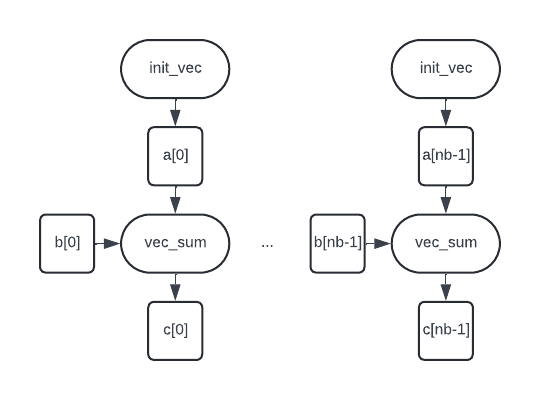
\includegraphics[scale=0.6]{fig_1.png}}
	\caption{Example numeric algorithm graph representation}
	\label{fig_1}
\end{figure}

In the figure, rectangles represent variables, ovals represent operations.

Consider another more complicated example.
The below code sample illustrates the description of sparse CSR matrix-vector product: \(y = A*x\), where 
\textit{x} is an input vector, \textit{A} is a CSR matrix and \textit{y} is an output vector storing the result. 
Vectors are represented as 1-dimensional arrays of vector blocks (each vector stores \textit{nb} vector blocks, each 
block is a 1-dimensional array of \textit{blockn} double precision floating point values). The input CSR matrix 
(\textit{A}) is represented as a 2-dimensional array of CSR blocks.
\begin{lstlisting}[frame=single]
//...

Array<int> ia[n+1];
Array<int> ja[nnz];
Array<double> a[nnz];

//...

BlockedCSRMatrix<double[][]> A = {n, n, 
	nnz, nb, nb, ia, ja, a};

Array<double[blockn]> x[nb];
Array<double[blockn]> y[nb];

//...

for (int i = 0; i < nb; ++i) {
	int v = 0;
	for (int j = 0; j < nb; ++j) {
		if (!%zero(A[i][j])) {
			csr_mv(nb, 
				blockn, 
				A[i][j], 
				x[j], 
				y{v}[i], 
				y{v+1}[i]);
			v = v + 1;
		}
	}
}
\end{lstlisting}

In the above example the input matrix is initialized using regular CSR arrays \textit{ia}, \textit{ja} and 
\textit{a}. Each CSR matrix block can be checked for emptiness by using \textit{\%zero} expression which is 
\textit{true} if the input CSR matrix block is empty and only stores zero values. The kernel \textit{csr\_mv} 
computes \( y[i] = y[i] + A[i][j] * x[i] \), where \textit{A[i][j]} is a CSR matrix block, 
\textit{y[i]} and \textit{x[i]} are the corresponding vector blocks. The use of two versions of each \textit{y[i]} vector 
block enables ParSolGen compiler to store the values of these formally independent vector blocks within the same 
memory location. This allows overwriting the values of \textit{y} vector reducing the potential run-time overhead 
introduced by the management of vector block instances.


\section{ParSolGen architecture}
ParSolGen consists of two main parts: a classifying compiler and a set of domain-specific run-time systems. 
ParSolGen compiler parses the input numerical algorithm description written in ParSolGen language and checks it 
for lexical and syntax errors. The it feeds the analyzed numerical algorithm description into 
the input of classifier. The classifier divides the input numerical algorithm description into non-intersecrting 
ordered subsets of ParSolGen language statements according to the class to which each statement belongs. Then 
the C++ parallel program is generated for each classified statements subset using the corresponding domain-specific 
code generation module. Each domain-specific code generation module is only suitable for a certain restricted 
numerical algorithms class (for example, for sparse linear algebra or stencil based numerical algorithms). 
The generated program can be 
linked to the corresponding domain-specific run-time systems if needed (for example, in case if static code generation is not possible or there is a need for dynamic load balancing support).
The process is illustrated in ``Fig.~\ref{fig_2}''.

\begin{figure}[htbp]
	\centerline{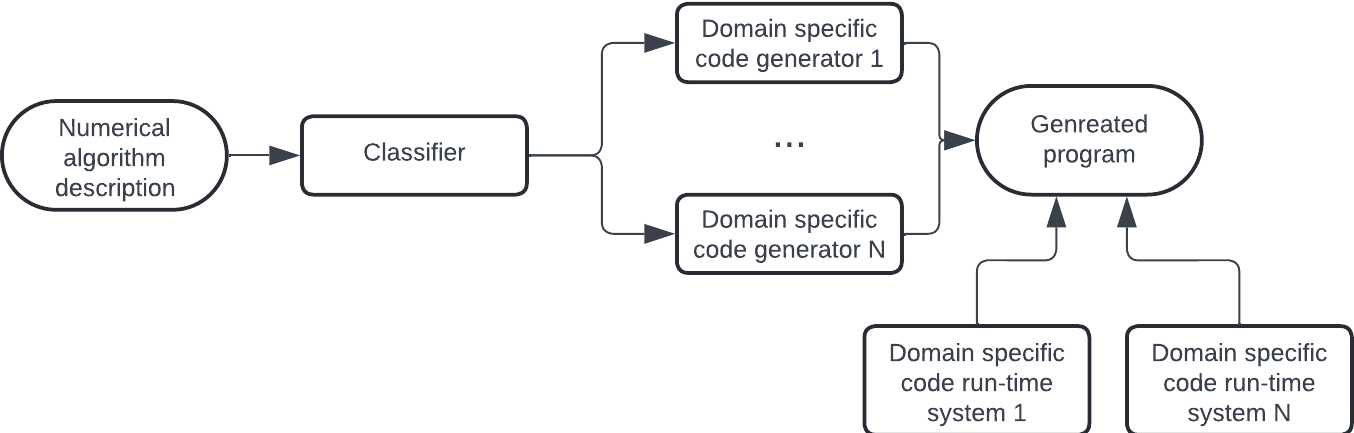
\includegraphics[width=8cm, height=3cm]{fig_2.png}}
	\caption{The process of parallel program construction in ParSolGen}
	\label{fig_2}
\end{figure}

\subsection{Numerical algorithm description classification}
ParSolGen compiler classifies the input numerical algorithm description by applying a set 
of the integrated domain-specific classification modules (one for each supported numerical algorithms class) to 
each statement. Each classification module (classifier) can determine if a statement belongs to the supported class. 
Let \(C_i\) be \textit{i}-th classifier and \(C_i(s) \in \{true, false\}\) denote the result of the application of 
classifier \(C_i\) to statement \(s \in S\) where \(S\) is an ordered set of ParSolGen statements representing the 
input numerical algorithm description in ParSolGen language. PsrSolGen classification algorithm is listed in ``Alg. \ref{alg:cap}''.
\begin{algorithm}
	\caption{An algorithm with caption}\label{alg:cap}
	\begin{algorithmic}
		\State $C \gets \{c_0, ..., c_m\}$ \Comment{Ordered set of the domain specific classifiers integrated to ParSolGen}
		\State $S \gets \{s_1, ..., s_n\}$ \Comment{Ordered set of ParSolGen statements representing the input numerical algorithm description}
		\State $R \gets \emptyset$ \Comment{Statements classification}
		\State $i \gets 1$ \Comment{Index of the current ParSolGen statement}
		\State $k \gets 1$ \Comment{Index of the current classifier}
		\While{$i \le |S|$}
		\State $s_i \gets next\ statement\ from\ S$
		\State $m \gets 1$
		\State $r \gets false $ \Comment{Result of the application of k-th classifier to i-th statement}
		\While{$m \le |C| \land r = false$}
		\If{$c_k(s_i) = true$}
		\State $R \gets R \cup \{ \langle s_i, k \rangle \} $
		\State $r \gets true$
		\Else
		\If{$k = |C|$}
		\State $k \gets 1$
		\Else
		\State $k \gets k + 1$
		\EndIf
		\EndIf
		\State $m \gets m + 1$
		\EndWhile
		\If{$r = false$}
		\Return{error} \Comment{\textit{i}-th statement is not classified - return error}
		\EndIf
		\State $i \gets i + 1$
		\EndWhile
	\end{algorithmic}
\end{algorithm}

The idea behind the classification algorithm is to find the domain-specific parallel program construction 
module which is suitable for the current statement. This is done by looping through all integrated classifiers 
until the \textit{k}-th classifier returns \textit{true}. If a statement cannot be classified an error is thrown and 
parallel program construction is aborted. 
Despite being trivial the above classification algorithm allows the accumulation of domain-specific 
classification and code generation modules in ParSolGen.

Each classification module implements a set of criteria which define a class of ParSolGen statements. 
For each class of statements supported by ParSolGen there is a classifier and a parallel program construction 
module. If a statement belongs to such supported statements class the corresponding parallel 
program construction module is used to generate a parallel program for the statement.

In this paper three statement classes are considered. The first supported statements class is 
referred as "dense linear algebra related statements class". ParSolGen statement is considered dense linear 
algebra statement if the following conditions are met:
\begin{itemize}
	\item sdss
\end{itemize}

It can be seen that the satisfaction of the above conditions does not necessarily guarantee 
that a statement describes a part of a dense linear algebra related algorithm. In case if a 
statement satisfies the above conditions, a parallel program for the statement will be constructed 
using the program construction module designed for dense linear algebra domain. 
In case of miss-classification the parallel program remains correct. However, in this case 
the domain-specific optimizations and technqiues employed in the process of the parallel 
program construction would potentially reduce the performance of the constructed parallel 
program. 

Consider the second supported statements class. It is referred to as "sparse linear algebra related statements class". 
The criteria defining this class are the following:
\begin{itemize}
	\item sdss
\end{itemize}
The notes provided for dense linear algebra-related statements also apply to the class described above. 

...
Vector algorithms class

The above criteria together define a ParSoGen numerical algorithm descriptions class which includes 
many dense and sparse linear algebra algorithms such as: dense \(LU, LL^T, LDL^T\) matrix factorization, various sparse iterative solver algorithms (Conjugated Gradient, Biconjugated gradient, Generalized Minimal Residual method etc.) and various sparse matrix preconditioner algorithms (Jacobi, Successive Over-Relaxation, etc.).

\section{ParSolGen parallel program construction}
Once the input algorithm description is classified a parallel program part is constructed 
for each classified statements subset. This is done by invoking the corresponding domain-specific 
parallel program construction modules which are integrated into ParSolGen compiler.  
For the dense and sparse linear algebra related numerical algorithms two staged parallel 
program construction process is applied. First so called \textit{intermediate} program is 
constructed for the corresponding subset of ParSolGen statements. The intermediate  
program builds graph representation of the ParSolGen statements subset at runtime. 
Then this graph representation is fed into the input of the domain-specific 
run-time system that executes it in a distributed manner. 
The process is illustrated in ``Fig.~\ref{fig_3}''

\begin{figure}[htbp]
	\centerline{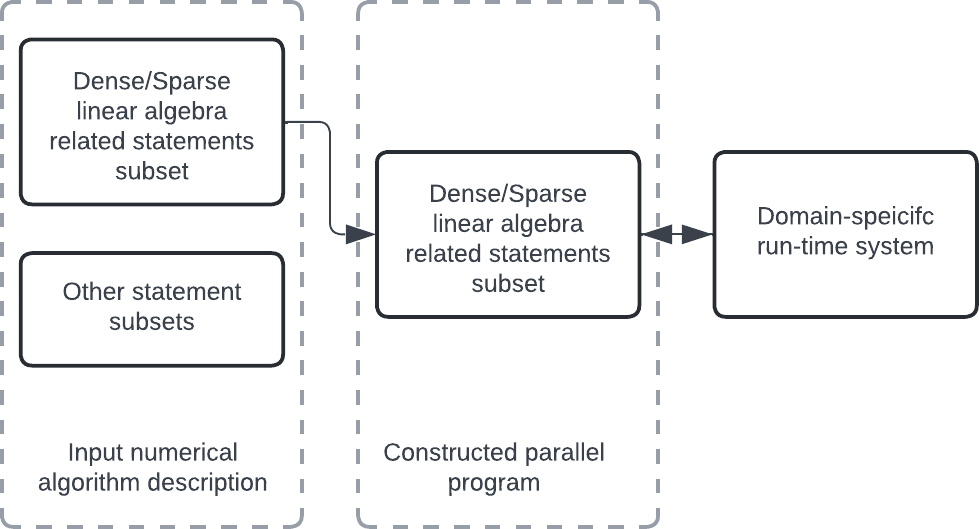
\includegraphics[width=8cm, height=4cm]{fig_3.png}}
	\caption{Two-staged parallel program construction process of dense and sparse linear algebra related algorithms}
	\label{fig_3}
\end{figure}

The domain-specific run-time system performs the distribution of the variables and operations 
of the input graph representation among the nodes of distributed memory parallel computer. 

\section{Performance evaluation}
The performance of the parallel programs constructed by ParSolGen is evaluated on four 
test applications: distributed dense matrix \(LL^T\) factorization, distributed sparse CSR 
matrix-vector product, distributed sparse CG (Conjugate Gradient) iterative solver and 
distributed sparse BiCG (Biconjugate Gradient) iterative solver. The parallel performance of 
the parallel programs constructed by ParSolGen was compared to that of the popular 
libraries implementing the same algorithms.

\subsection{Distributed dense matrix \(LL^T\) factorization}
A parallel program was constructed by the ParSolGen description of algorithm of 
\(LL^T\) factorization of a dense matrix. The performance of the parallel program 
constructed by ParSolGen was compared to that of ScaLAPACK (v2.2.0) implementation of \(LL^T\) 
factorization. 

\subsection{Parallel sparse matrix-vector product}
The performance of the parallel program constructed by ParSolGen from CSR matrix-vector 
product description is compared to that of Intel MKL (v2021.4.0) on single node 
(Intel 12th Gen Intel(R) Core(TM) i7-12700H, 64GB RAM). The test was performed on 
"VLSI/stokes" CSR matrix from the Sparse Matrix Collection \cite{spcol}. 
The input double precision CSR matrix was represented 
as a 2-dimensional ParSolGen array of CSR matrix blocks. Both generated program and Intel 
MKL implementation performed 1000 sparse matrix vector product operations and the execution 
time was measured.
The results are depicted in ``Fig.~\ref{fig_perf_spmv_mkl}''.
\begin{figure}[htbp]
	\centerline{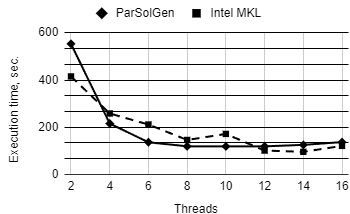
\includegraphics[scale=0.8]{fig_perf_spmv_mkl.png}}
	\caption{The process of parallel program construction in ParSolGen}
	\label{fig_perf_spmv_mkl}
\end{figure}
Here the performance of the parallel program constructed by ParSolGen is comparable to 
that of Intel MKL implementation.

\subsection{}

\section{Conclusion}
Automatic parallel program construction requires different construction system algorithms 
and techniques for different subject domains. ParSolGen is designed for accumulation of 
various domain-specific automatic parallel program construction algorithm. This ability 
was demonstrated by accumulating specialized parallel program construction algorithms for 
dense and sparse linear algebra domains into ParSolGen. The performance of the parallel 
programs automatically constructed by ParSolGen from the description of 
sparse matrix-vector product, dense \(LL^T\) matrix factorization, sparse CG (Conhugated Gradient) and 
sparse BiCG (Biconjugate gradient) algorithms is comparable to that of widely used libraries. 
This makes ParSolGen a practically useful tool for the automatic construction of highly efficient 
distributed parallel programs for sparse iterative solvers and dense linear algebra subject domains. 
Other numerical algorithm classes can also be supported by ParSolGen by integrating the corresponding 
domain specific parallel program construction algorithms.


\begin{thebibliography}{00}
\bibitem{legion} Bauer, Michael, et al. "Legion: Expressing locality and independence with logical regions." SC'12: Proceedings of the International Conference on High Performance Computing, Networking, Storage and Analysis. IEEE, 2012.
\bibitem{charm} Kale, Laxmikant V., and Sanjeev Krishnan. "Charm++ a portable concurrent object oriented system based on c++." Proceedings of the eighth annual conference on Object-oriented programming systems, languages, and applications. 1993.
\bibitem{charm1} Kale, Laxmikant V., and Sanjeev Krishnan. "Charm++." (1996).
\bibitem{quark} AsimYarkhan.2012. DynamicTaskExecutiononSharedandDistributedMemory Architectures. December (2012). http://trace.tennessee.edu/utk
\bibitem{starpu} Augonnet, Cédric, Samuel Thibault, and Raymond Namyst. StarPU: a runtime system for scheduling tasks over accelerator-based multicore machines. Diss. INRIA, 2010.
\bibitem{halide} Ragan-Kelley, Jonathan, et al. "Halide: a language and compiler for optimizing parallelism, locality, and recomputation in image processing pipelines." Acm Sigplan Notices 48.6 (2013): 519-530.
\bibitem{dplasma} Bosilca, George, et al. "Flexible development of dense linear algebra algorithms on massively parallel architectures with DPLASMA." 2011 IEEE International Symposium on Parallel and Distributed Processing Workshops and Phd Forum. IEEE, 2011.
\bibitem{dague} Bosilca, George, et al. "DAGuE: A generic distributed DAG engine for high performance computing." Parallel Computing 38.1-2 (2012): 37-51.
\bibitem{regent} Slaughter, Elliott. Regent: A high-productivity programming language for implicit parallelism with logical regions. Diss. Stanford University, 2017.
\bibitem{regent1} Slaughter, Elliott, et al. "Regent: a high-productivity programming language for HPC with logical regions." Proceedings of the International Conference for High Performance Computing, Networking, Storage and Analysis. 2015.
\bibitem{luna} Belyaev, Nikolay, and Vladislav Perepelkin. "High-efficiency specialized support for dense linear algebra arithmetic in LuNA system." Parallel Computing Technologies: 16th International Conference, PaCT 2021, Kaliningrad, Russia, September 13–18, 2021, Proceedings 16. Springer International Publishing, 2021.
\bibitem{luna1} Belyaev, Nikolay, and Vladislav Perepelkin. "High-efficiency specialized support for dense linear algebra arithmetic in LuNA system." Parallel Computing Technologies: 16th International Conference, PaCT 2021, Kaliningrad, Russia, September 13–18, 2021, Proceedings 16. Springer International Publishing, 2021.
\bibitem{spcol} Davis, Timothy A., and Yifan Hu. "The University of Florida sparse matrix collection." ACM Transactions on Mathematical Software (TOMS) 38.1 (2011): 1-25.
\end{thebibliography}

\vspace{12pt}
\color{red}
IEEE conference templates contain guidance text for composing and formatting conference papers. Please ensure that all template text is removed from your conference paper prior to submission to the conference. Failure to remove the template text from your paper may result in your paper not being published.

\end{document}
